Um den Umgang mit Tkinter zu �ben, werden wir eine einfache Anwendung zum Anzeigen
von geometrischen Figuren programmieren. Diese Anwendung wird unter anderem aus einem Listen-Widget,
mehrerer Buttons, einem Canvas-Widget, sowie einem Popup-Fenster mit Labels und
Eingabe-Widgets bestehen. Es ist sinnvoll die vorherigen Aufgaben bearbeitet
und ein grundlegendes Verst�ndnis f�r Klassen und Funktionen in Python zu haben.
Das Listen-Widget wird die Namen der geometrischen Figuren enthalten. �ber Buttons
k�nnen neue Figuren angelegt oder bestehende gel�scht werden. Ist eine Figur aus
der Liste ausgew�hlt, kann diese �ber einen Button auf das Canvas-Widget gezeichnet werden.
Ein weiterer Button l�scht die Anzeigefl�che des Canvas-Widget. Das folgende Bild beschreibt
einen m�glichen Aufbau der Anwendung:

\begin{figure}[ht]
	\centering
	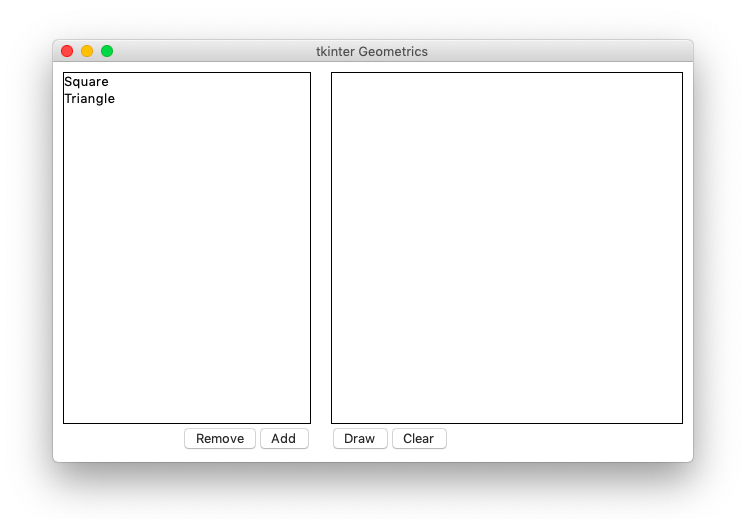
\includegraphics[width=0.5\textwidth]{images/GeometricsGUI.png}
	\caption{Auf der linken Seite befindet sich das Listen-Widget, sowie zweit Buttons 'Add' und 'Remove'.
  Auf der rechten Seite das Canvas-Widget und zwei Buttons 'Draw' und 'Clear'.}
	\label{fig:GeometricsGUI}
\end{figure}

Legen Sie als Erstes zwei Frame-Widgets mit dem Namen Left- und RightFrame an. �bergeben Sie
diese anschlie�end dem Fenster, so dass es in zwei gleichgro�e Sektionen
unterteilt wird.
